\chapter{引言}
\section{研究背景和意义}
地震勘探的终极目标是通过观测到地震数据来定量地估计地下模型。
弹性参数,包括纵(P)波速度,横(S)波速度以及密度等等物性参数可以通过岩石物理来定量的估计岩石物理参数,从而获得储层及其围岩的岩石性质。这对油气的开发,油田
监测以及CO$_2$注入等具有重要意义。传统的常规地震数据处理中,通常用声波方程来描述地震波在地下介质中的传播。而地下介质的真实模型往往要复杂得多,需要通过弹性
各向同性、具有垂直(水平)对称轴的横向各向同性(VTI,HTI)、正交各向异性(ORT)、衰减等等来更准确的描述波传播。但是模型假设越复杂,所引入的计算量也越大,
而所对应的多参数反问题也越困难。目前来看从声介质过渡到弹性介质能够以较小代价来获取较准确的模型近似。
尽管如此,从声波近似过渡到到弹性假设也会成倍地增加计算量,但是采用弹性波假设来进行成像或者反演仍然十分必要。因为考虑弹性假设的数据处理流程能区分数据中的
P波与S波模式,从而获得更多与岩性相关的信息,这对于岩性估计、流体识别、气云成像、裂缝与应力刻画以及密度估计都非常重要。
近年来,非常规油气藏,如致密页岩气(油)等开发技术极大地依赖于岩石物理参数的估计,这使得考虑弹性介质甚至各向异性假设都需要提上日程。

地震勘探中的诸多技术都非常依赖于速度模型的精度。
因此在众多物性参数中,如何获取准确的高分辨率速度模型是地震勘探中最为迫切的任务。
为了降低地震数据与模型描述之间的非线性程度,Claerbout(1985)\cite{Claerbout1985Imaging}在其书中将速度模型分解为两个部分:1)描述速度(阻抗)界面的高频部分;
2)描述波传播走时的低频部分。这样的分解方式分别对应于地震勘探中最核心的两个任务,也即偏移成像与速度建模。传统方法中偏移成像+AVO/AVA
技术通常用来获取模型的高频部分,
而偏移速度分析(MVA)和层析技术被用来恢复模型的低频部分。但是这类方法所能恢复的波数谱上存在明显的间断区域,正如著名的图\ref{fig:GapInSeisVel}
所示(选自Claerbout(1985)\cite{Claerbout1985Imaging}),速度模型的中低成分波数很难恢复。而随着高性能计算能力的不断提升,
基于波动理论来获取模型高频和低频波数部分受到了广泛关注。

\begin{figure}[!htb] 
   \centering 
   \subfloat[]{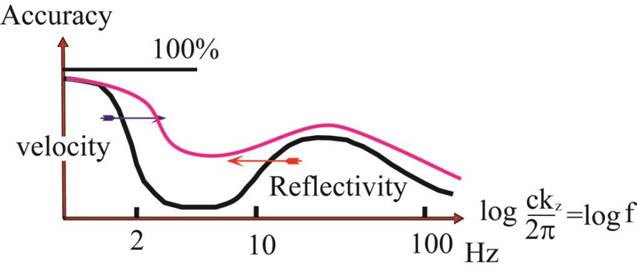
\includegraphics[width=0.68\textwidth]{Figure/chapter01/GapInSeis.jpg}}
   \caption{Vertical profiles of elastic WERTI and EFWI results at 1.4km (a) and
       3km (b). The black and blue lines indicate the true and linearly         increased
       initial model. The green and yellow lines indicate the WERTI and EFWI    results,
       respectively.
   }
   \label{fig:GapInSeisVel}
\end{figure}
目前
地震勘探中深度域偏移成像质量非常依赖于速度模型的精度。且随着勘探的发展,成像技术中越来越需要考虑各向异性,而在各向异性介质中,成像则更加
依赖各向异性参数的准确性。因而需要考虑各向异性介质中的深度域建模。此外,基于层析的建模方法只能提供较好的偏移模型,但是地震勘探中我们总希
望得到对地下介质更为精细的刻画,这就需要引入全波形反演技术(FWI)。传统的FWI方法中通常基于拟声波方程来描述波场,这与地下介质的弹性假设并
不相符,近年来由于计算机能力提升、多分量观测数据的增多以及解决声波FWI无法回避的问题的需要,考虑弹性甚至各向异性的全波形反演逐渐成为研究热
点。弹性波多分量数据中同时含有纵波(P波)和横波(S波),这两种不同波模式对地下介质有着不同的刻画作用。近年来弹性波波模式分离技术能够提供准
确的P或S波数据,这将会对反演带来许多有益的帮助。此外,反射全波形反演(RWI)通过反射波信息来建立初始模型。对于弹性波RWI,模式解耦提供的分
离的P或S波数据同样会非常有帮助。
\section{研究现状}
\subsection{弹性波FWI研究现状}
\subsection{弹性反射波FWI研究现状}
\subsection{弹性波LSRTM研究现状}
\section{研究内容}
